\section{Fourier Transforms} \label{sec:fourier}

\subsection{Eigenfunctions and $H(s)$}

An \emph{eigenfunction} $x(t) = e^{j\omega t}$ is a function such that
$S\{x(t)\} = Ax(t)$ for LTI $S$. A property of functions of the form
$e^{j\omega t}$ is that convolution with $h(t)$ yields
\begin{equation}
    x(t) * h(t) = e^{j\omega t} \int_{-\infty}^{\infty} h(\tau) e^{-j\omega \tau} d\tau.
\end{equation}
This is also written as
\begin{equation}
    x(t) * h(t) = e^{j\omega t} \left( |H(j\omega)|e^{j \angle H(j\omega)} \right)
\end{equation}
$H$ is known as the transfer function as has the property that
$Y(S) = H(s)X(s)$, where $Y(s)$ and $X(s)$ are the Laplace transforms
of $y(t)$ and $x(t)$.

\section{Fourier Series}

Consider an arbitrary periodic CT signal $x(t)$ with fundemental
period $T$ and fundemental frequency $\omega_0$. The Fourier series
representation of $x(t)$ is
\begin{align}\label{eq:synthesis}
    x(t) & = \sum_{k=-\infty}^{\infty} a_k e^{jk\omega_0 t}                           \\
         & = a_0 + a_1e^{j\omega_0 t} + a_{-1}e^{-j\omega_0 t} + a_2e^{2j\omega_0 t},
\end{align}
where $a_k$ is the $k$th Fourier coefficient and can be found with the formula
\begin{equation}
    a_k = \frac{1}{T} \int_{<T>} x(t) e^{-jk\omega_0 t} dt
\end{equation}
with $<T>: [0, T], [-\frac{T}{2}, \frac{T}{2}, ...]$.
Equation \ref{eq:synthesis} is known as the synthesis equation. The process of
of finding $a_k$ is Fourier analysis.

Notably, $a_0$ gives the DC component of the singal. In general the $a_{\pm k}$
are the $k$th harmonic components.

Let's see an example. Let $x(t)$ be a square wave given by
\begin{equation}
    x(t) = \begin{cases}
        1 & |t| < T_1               \\
        0 & T_1 < |t| < \frac{T}{2}
    \end{cases}
\end{equation}

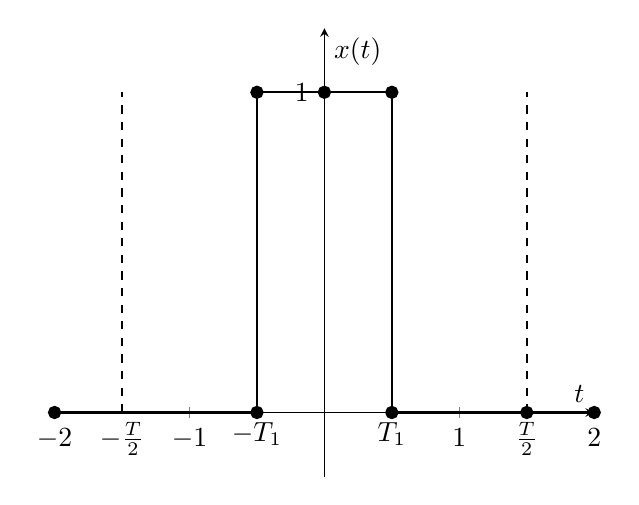
\begin{tikzpicture}
    \begin{axis}[
            axis x line=middle,
            axis y line=middle,
            xlabel={$t$},
            ylabel={$x(t)$},
            xtick={-2, -1, 0, 1, 2},
            ytick={0, 1},
            ymin=-0.2, ymax=1.2,
            xmin=-2, xmax=2,
            samples=100,
            domain=-2:2,
        ]
        \addplot[
            domain=-2:2,
            samples at={-2,-1.5,-1, -0.5, 0, 0.5, 1, 1.5, 2},
            mark=*,
            thick
        ] coordinates {(-2,0) (-0.5,0) (-0.5,1) (0,1) (0.5,1) (0.5,0) (1.5,0) (2,0)};

        \addplot[dashed, thick] coordinates {(-0.5,0) (-0.5,1)};
        \addplot[dashed, thick] coordinates {(0.5,0) (0.5,1)};
        \addplot[dashed, thick] coordinates {(1.5,0) (1.5,1)};
        \addplot[dashed, thick] coordinates {(-1.5,0) (-1.5,1)};

        \node[anchor=north] at (axis cs:-0.5,0) {$-T_1$};
        \node[anchor=north] at (axis cs:0.5,0) {$T_1$};
        \node[anchor=north] at (axis cs:1.5,0) {$\frac{T}{2}$};
        \node[anchor=north] at (axis cs:-1.5,0) {$-\frac{T}{2}$};
    \end{axis}
\end{tikzpicture}

We calculate $a_k$ as
\begin{align}
    a_k & = \frac{1}{T} \int_{<T>} x(t) e^{-jk\omega_0 t} dt                                         \\
        & = -\frac{1}{jk\omega_0 T} \left[ e^{-jk\omega_0 T_1} -  e^{jk\omega_0 T_1}\right]          \\
        & = \frac{1}{k\omega_0 T} \left[ \frac{e^{jk\omega_0 T_1} -  e^{-jk\omega_0 T_1}}{j} \right] \\
        & = \frac{2}{omega_0 T} \sin(k \omega_0 T_1)                                                 \\
        & = \frac{1}{\pi k} \sin(k \omega_0 T_1)
\end{align}
This expression for $a_0$ is fine, however, there is a problem. When
$k = 0$ we have a discontinuity. In general we may have to find $a_0$
separately. It's not a big deal: $a_0 = \frac{1}{T} \int_{-T_1}^{T_1} 1 dt$.

$a_k$ as a function of $k$ given the \emph{spectrum} of $x(t)$. Let's see
an example: let $T_1 = \frac{T}{4}$. Then $a_k = \frac{\sin(\pi \frac{k}{2})}{k\pi}$.

\begin{tikzpicture}
    \begin{axis}[
            axis x line=middle,
            axis y line=middle,
            xlabel={$t$},
            ylabel={$x(t)$},
            xtick={-2, -1, 0, 1, 2},
            ytick={0, 1},
            ymin=-0.2, ymax=1.2,
            xmin=-2, xmax=2,
            samples=100,
            domain=-2:2,
        ]
        \addplot[
            domain=-2:2,
            samples at={-2,-1.5,-1, -0.5, 0, 0.5, 1, 1.5, 2},
            only marks
        ] coordinates {((0,0.5) ((1,0.32) (-1, 0.32) (-2,0) (3, -0.1) (-3, -0.1) };
    \end{axis}
\end{tikzpicture}